\documentclass[a5paper,twoside,openright]{article} % twoside permet d'avoir le décalage fait exprès
\usepackage[utf8]{inputenc}
\usepackage[french]{babel}
\usepackage[T1]{fontenc}
\usepackage[final]{pdfpages}
\usepackage{graphicx}
\usepackage{scrextend} % to specify indent
\usepackage{sectsty} % to change color of section headings
\usepackage{tikz} % to wrap text around figures
\usepackage{svg} % to svg
\usepackage{calc} % to svg
\usepackage[explicit]{titlesec} % to add two-side reference with toc and sections
\usepackage{titletoc} % multiple categories
\usepackage{pgffor} % foreach
\usepackage{multicol} % Allow multicolums
\usepackage{ifthen}
\usepackage{etoolbox} % to handle lists
\usepackage{attachfile} % to handle embedded audios
\usepackage[paper, colored, categories]{tagging} 
% paper = chant to print
% onlineOnly = chant not to print
% partition = to show partitions for chants that have one
% colored = shows colors on chant pages
% categories = to show toc by categories
\usepackage[top=2cm, bottom=2cm]{geometry}
% Marges suffisantes ?
%\geometry{height=23cm,width=16cm}
\geometry{hmargin={3cm,1.5cm}}
\geometry{vmargin={1.5cm,2cm}}
\usepackage{hyperref} % gestion des hyperliens dans la table des matieres
\usepackage{yfonts} % support for old german fonts
\usepackage{lettrine} % Enluminures
\input Romantik.fd % Enluminures

%% CATEGORIES %%
%% Using an optional argument other than c in \header allow a horizontal spanning of categories

\listgadd\categories{}

\newcommand{\newCategory}[1]{\startcontents[#1]\stopcontents[#1]}
\newcommand{\printCategory}[2]{
    \dualcol{
        \printcontents[#1]{l}{1}{
            \renewcommand{\baselinestretch}{0.75}\normalsize
            % \let\section\oldsection
            % \pdfbookmark{Contents}{Contents}
            \section*{#2}\setcounter{tocdepth}{1}
            \renewcommand{\baselinestretch}{1.0}\normalsize
        }
    }
}


\newcommand{\splitCategories}[1]{
    \ifthenelse{\equal{\arabic{valuex}}{2}}{
        \setcounter{valuex}{0}
        \stepcounter{valuey}
    }{}
    \ifthenelse{\equal{\arabic{valuey}}{0}}{
        \ifthenelse{\equal{\arabic{valuex}}{0}}{
            \listgadd{\rowOneColumnOne}{#1}
        }{
            \listgadd{\rowOneColumnTwo}{#1}
        }
    }{
        \ifthenelse{\equal{\arabic{valuex}}{0}}{
            \listgadd{\rowTwoColumnOne}{#1}
        }{
            \listgadd{\rowTwoColumnTwo}{#1}
        }
    }
    \stepcounter{valuex}
    \stepcounter{lengh}
}%

\newcommand{\removeCategories}[1]{
    \ifthenelse{\equal{\arabic{valuex}}{2}}{
        \setcounter{valuex}{0}
        \stepcounter{valuey}
    }{}
    \ifthenelse{\equal{\arabic{valuey}}{0}}{
        \ifthenelse{\equal{\arabic{valuex}}{0}}{
            \listgremove{\rowOneColumnOne}{#1}
        }{
            \listgremove{\rowOneColumnTwo}{#1}
        }
    }{
        \ifthenelse{\equal{\arabic{valuex}}{0}}{
            \listgremove{\rowTwoColumnOne}{#1}
        }{
            \listgremove{\rowTwoColumnTwo}{#1}
        }
    }
    \stepcounter{valuex}
    \stepcounter{lengh}
}%

\newcounter{lengh}
\newcounter{valuex}
\newcounter{valuey}
\newcommand{\insertCategories}[1]{
    \forcsvlist{\listgadd{\rowOneColumnOne}}{}
    \forcsvlist{\listgadd{\rowOneColumnTwo}}{}
    \forcsvlist{\listgadd{\rowTwoColumnOne}}{}
    \forcsvlist{\listgadd{\rowTwoColumnTwo}}{}
    \forlistloop{\splitCategories}{\categories}
    \setcounter{valuex}{0}
    \setcounter{valuey}{0}
    \parseCategories{\rowOneColumnOne}{\rowOneColumnTwo}{\rowTwoColumnOne}{\rowTwoColumnTwo}{#1}
    \forlistloop{\removeCategories}{\categories}
    \setcounter{valuex}{0}
    \setcounter{valuey}{0}
    \setcounter{lengh}{0}
}

\newcommand{\showCategory}[1]{
    \hyperref[sec:#1]{\includegraphics[scale=0.3]{images/categories/#1.png}}
}

\newcommand{\showCategories}[2]{
    \ifthenelse{\equal{#1}{c}}{
        \begin{tabular}{cc}
            #2
        \end{tabular}
    }{
        \ifthenelse{\equal{#1}{v}}{
            \begin{tabular}{c}
                #2
            \end{tabular}
        }{
            \begin{tabular}{cccc}
                #2
            \end{tabular}
        }
    }
}

\newcommand{\showCategoriesOne}[1]{
    \showCategories{#1}{
        & \forlistloop{\showCategory}{\rowOneColumnOne}
    }
}

\newcommand{\showCategoriesTwo}[1]{
    \ifthenelse{\equal{#1}{v}}{
        \showCategories{#1}{
            \forlistloop{\showCategory}{\rowOneColumnOne} \vspace{0.3cm}\\
            \forlistloop{\showCategory}{\rowOneColumnTwo} \vspace{0.3cm}\\
        }
    }{
        \showCategories{#1}{
        \forlistloop{\showCategory}{\rowOneColumnOne} &
        \forlistloop{\showCategory}{\rowOneColumnTwo}
        }
    }
}

\newcommand{\showCategoriesThree}[1]{
    \ifthenelse{\equal{#1}{c}}{
        \showCategories{#1}{
            \forlistloop{\showCategory}{\rowOneColumnTwo} &
            \forlistloop{\showCategory}{\rowOneColumnOne} \vspace{0.3cm}\\
            & \forlistloop{\showCategory}{\rowTwoColumnOne}
        }
    }{
        \ifthenelse{\equal{#1}{v}}{
            \showCategories{#1}{
                \forlistloop{\showCategory}{\rowOneColumnTwo} \vspace{0.3cm}\\
                \forlistloop{\showCategory}{\rowOneColumnOne} \vspace{0.3cm}\\
                \forlistloop{\showCategory}{\rowTwoColumnOne} \vspace{0.3cm}\\
            }
        }{
            \showCategories{#1}{
                & \forlistloop{\showCategory}{\rowOneColumnTwo} &
                \forlistloop{\showCategory}{\rowOneColumnOne} &
                \forlistloop{\showCategory}{\rowTwoColumnOne}
            }
        }
    }
}


\newcommand{\showCategoriesFour}[1]{
    \ifthenelse{\equal{#1}{c}}{
        \showCategories{#1}{
            \forlistloop{\showCategory}{\rowOneColumnTwo} &
            \forlistloop{\showCategory}{\rowOneColumnOne} \vspace{0.3cm}\\
            \forlistloop{\showCategory}{\rowTwoColumnTwo} &
            \forlistloop{\showCategory}{\rowTwoColumnOne}
        }
    }{
        \ifthenelse{\equal{#1}{v}}{
            \showCategories{#1}{
                \forlistloop{\showCategory}{\rowOneColumnTwo} \vspace{0.3cm}\\
                \forlistloop{\showCategory}{\rowOneColumnOne} \vspace{0.3cm}\\
                \forlistloop{\showCategory}{\rowTwoColumnTwo} \vspace{0.3cm}\\
                \forlistloop{\showCategory}{\rowTwoColumnOne} \vspace{0.3cm}\\
            }
        }{
            \showCategories{#1}{
                \forlistloop{\showCategory}{\rowOneColumnTwo} &
                \forlistloop{\showCategory}{\rowOneColumnOne} &
                \forlistloop{\showCategory}{\rowTwoColumnTwo} &
                \forlistloop{\showCategory}{\rowTwoColumnOne}
            }
        }
    }
}

\newcommand{\parseCategories}[5]{
    \ifthenelse{\equal{\arabic{lengh}}{0}}{}{
        \ifthenelse{\equal{\arabic{lengh}}{1}}{
            \showCategoriesOne{#5}
        }{
            \ifthenelse{\equal{\arabic{lengh}}{2}}{
                \showCategoriesTwo{#5}
            }{
                \ifthenelse{\equal{\arabic{lengh}}{3}}{
                    \showCategoriesThree{#5}
                }{
                    \ifthenelse{\equal{\arabic{lengh}}{4}}{
                        \showCategoriesFour{#5}
                    }{}
                }
            }
        }
    }
}

%% GENERAL %%
\newcommand{\enluminure}[3]{\lettrine[lines=#1]{\usefont{U}{Romantik}{xl}{n} #2}{#3}}

\setlength\parindent{0pt}

\newcommand{\breakpage}{\newpage}

\newcommand{\newSection}[1]{
  \thispagestyle{empty}
  \vspace*{200pt}\par
  {\Huge \centering \bfseries #1\par\nobreak
  \vskip 100pt}
  \breakpage
}

\newcommand{\dualcol}[1]{
    \begin{multicols}{2}
        #1
    \end{multicols}
}


\newcommand{\blackline}[0]{
    \vspace{1cm}
    \hrule
    \vspace{1cm}
}

\newcommand{\bissimple}[1][]{\} bis}

\newcommand{\bisdouble}[2]{
    % The spaces are NECESSARY DON'T ERASE THEM

    % \ensuremaths{
    %     \left.
    %     \hspace{-0.25cm}
    %     \begin{tabular}{l}
    %     #1
    %     \\#2
    %     \end{tabular}\right\rbrace
    % } \textrm{bis}

    $\left.
    \hspace{-0.25cm}
    \begin{tabular}{l}
    #1
    \\#2
    \end{tabular}\right\rbrace$ \textrm{bis}
    
    % The spaces are NECESSARY DON'T ERASE THEM
}

\newcommand{\bisdoublespace}[2]{
    % The spaces are NECESSARY DON'T ERASE THEM

    % \ensuremaths{
    %     \left.
    %     \hspace{-0.25cm}
    %     \begin{tabular}{l}
    %     #1
    %     \\#2
    %     \end{tabular}\right\rbrace
    % } \textrm{bis}\\
    % \vspace{0.2cm}

    $\left.
    \hspace{-0.25cm}
    \begin{tabular}{l}
    #1
    \\#2
    \end{tabular}\right\rbrace$ \textrm{bis}\\
    \vspace{0.2cm}
    
    % The spaces are NECESSARY DON'T ERASE THEM
}

\newcommand{\bistriple}[3]{
    % The spaces are NECESSARY DON'T ERASE THEM
    
    $
        \left.
        \hspace{-0.25cm}
        \begin{tabular}{l}
        #1
        \\#2
        \\#3
        \end{tabular}\right\rbrace
    $ \textrm{bis}
    
    % The spaces are NECESSARY DON'T ERASE THEM
}

\newcommand{\bistriplespace}[3]{
    % The spaces are NECESSARY DON'T ERASE THEM

    $
        \left.
        \hspace{-0.25cm}
        \begin{tabular}{l}
        #1
        \\#2
        \\#3
        \end{tabular}\right\rbrace
    $ \textrm{bis}\\
    \vspace{0.2cm}
    
    % The spaces are NECESSARY DON'T ERASE THEM
}

\newcommand{\bisquadruple}[4]{
    % The spaces are NECESSARY DON'T ERASE THEM

    $
        \left.
        \hspace{-0.25cm}
        \begin{tabular}{l}
        #1
        \\#2
        \\#3
        \\#4
        \end{tabular}\right\rbrace
    $ \textrm{bis}
    
    % The spaces are NECESSARY DON'T ERASE THEM
}

\newcommand{\bisquadruplespace}[4]{
    % The spaces are NECESSARY DON'T ERASE THEM

    $
        \left.
        \hspace{-0.25cm}
        \begin{tabular}{l}
        #1
        \\#2
        \\#3
        \\#4
        \end{tabular}\right\rbrace
    $ \textrm{bis}\\
    \vspace{0.2cm}
    
    % The spaces are NECESSARY DON'T ERASE THEM
}

\newcommand{\bisquintuple}[5]{
    % The spaces are NECESSARY DON'T ERASE THEM

    $
        \left.
        \hspace{-0.25cm}
        \begin{tabular}{l}
        #1
        \\#2
        \\#3
        \\#4
        \\#5
        \end{tabular}\right\rbrace
    $ \textrm{bis}
    
    % The spaces are NECESSARY DON'T ERASE THEM
}

\newcommand{\bisquintuplespace}[5]{
    % The spaces are NECESSARY DON'T ERASE THEM

    $
        \left.
        \hspace{-0.25cm}
        \begin{tabular}{l}
        #1
        \\#2
        \\#3
        \\#4
        \\#5
        \end{tabular}\right\rbrace
    $ \textrm{bis}\\
    \vspace{0.2cm}
    
    % The spaces are NECESSARY DON'T ERASE THEM
}

%% HEADER MANAGEMENT %%
%% Using an optional argument other than c in \header allow a horizontal spanning of categories instead of a square one

\newcommand{\header}[2][c]{
    \ifthenelse{\equal{#1}{c}}{
        \begin{minipage}[t]{.77\textwidth}
            \kern0pt
            #2
        \end{minipage}
        \hfill
        \hspace{0.5cm}
        \begin{minipage}[t]{.2\textwidth}
            \kern0pt
            \insertCategories{#1}
        \end{minipage}
    }{
        \ifthenelse{\equal{#1}{v}}{
            \begin{minipage}[t]{.85\textwidth}
                \kern0pt
                #2
            \end{minipage}
            \hfill
            \hspace{0.5cm}
            \begin{minipage}[t]{.15\textwidth}
                \kern0pt
                \insertCategories{#1}
            \end{minipage}
        }{
            \begin{minipage}[t]{.6\textwidth}
                \kern0pt
                #2
            \end{minipage}
            \hfill
            \hspace{0.5cm}
            \begin{minipage}[t]{.4\textwidth}
                \kern0pt
                \insertCategories{#1}
            \end{minipage}
        }
    }
    %\vspace{0.2cm}
}

\renewcommand{\LettrineTextFont}{}

%% COMMENTARY MANAGEMENT

\newcommand{\insertComment}[2]{
    \ifthenelse{\equal{#1}{}}{
        \ifthenelse{\equal{#2}{}}{
        }{
            \subsection{#2}
        }
    }{
        \ifthenelse{\equal{#2}{}}{
            \subsection{#1}
        }{
            \subsection{#1\\#2}
        }
    }
}

%% PDF MANAGEMENT

% \hypersetup{
%     colorlinks,
%     linkcolor={},
%     citecolor={},
%     urlcolor={}
% }

%% SECTION TITLE MANAGEMENT %%

% renew \section to link to the toc

% \let\oldcontentsline\contentsline%
% \renewcommand\contentsline[4]{%
% \hypertarget{toc#4}{}%
% \oldcontentsline{#1}{#2}{#3}{#4}}
% \let\oldsection\section
% \renewcommand\section[1]{%
%     \oldsection[#1]{\protect\hyperlink{toc}{#1}}}

% \let\oldsection\section
% \renewcommand{\section}{\protect\hyperlink{toc{\oldsection}}

% \titleformat{\chapter}[display]
% {\normalfont\huge\bfseries}{\chaptertitlename\ \thechapter}{20pt}{\Huge\hyperlink{toc}}
% \titleformat{\section}
% {\normalfont\Large\bfseries}{\thesection}{1em}{\hyperlink{toc}}
% \titleformat{name=\section, numberless}
% {\normalfont\Large\bfseries}{}{0em}{\hyperlink{toc}}
% \titleformat{\subsection}
% {\normalfont\large\bfseries}{\thesubsection}{1em}{\hyperlink{toc}}
% \titleformat{\subsubsection}
% {\normalfont\normalsize\bfseries}{\thesubsubsection}{1em}{\hyperlink{toc}}

\newcommand{\headtitle}[1]{
    \phantomsection
    % \addcontentsline{toc}{section}{#1} 
    % {\normalfont\Large\bfseries \protect\hyperlink{toc}{#1}}
    \section{\protect\hyperlink{toc}{#1}}
    % \section{#1}
}
%% COLOR MANAGEMENT %%
\newcounter{color}
\definecolor{falRoyalBlue}{RGB}{65,105,225}
\definecolor{falGreen}{RGB}{0,128,0}
\definecolor{falFuchsia}{RGB}{199,21,133}
\definecolor{falRed}{RGB}{220,20,60}
\definecolor{falPink}{RGB}{255,192,203}
\definecolor{falGrey}{RGB}{176,196,222}
\definecolor{falPurple}{RGB}{148,0,211}


\definecolor{color0}{RGB}{240,128,128} % light coral
\definecolor{color1}{RGB}{222,184,135} % burly wood
\definecolor{color2}{RGB}{123,104,238} % medium slate blue
\definecolor{color3}{RGB}{50,205,50} % lime green
\definecolor{color4}{RGB}{218,112,214} % orchid
\definecolor{color5}{RGB}{189,183,107} % dark khaki
\definecolor{color6}{RGB}{255,140,0} % dark orange
\definecolor{color7}{RGB}{72,209,204} % medium turquoise
\definecolor{color8}{RGB}{107,142,35} % olive drab
\definecolor{color9}{RGB}{0,128,128} % teal

%% CHANTS %%

\newcommand{\insertChant}[3]{
    \tagged{#2}{
        \ifthenelse{\equal{9}{\value{color}}}{
            \setcounter{color}{0}
        }{
            \stepcounter{color}
        }
        \tagged{colored}{
            \sectionfont{\color{color\arabic{color}!60!black}} 
            \subsectionfont{\fontsize{8}{10}\bfseries\itshape\color{color\arabic{color}!80!white}} 
            \renewcommand\LettrineFontHook{\color{color\arabic{color}}}%
        }
        \untagged{colored}{
            \sectionfont{\color{black}} 
            \subsectionfont{\fontsize{8}{10}\bfseries\itshape\color{black}} 
            \renewcommand\LettrineFontHook{\color{black}}%
        }
        \ifthenelse{\equal{#3}{}}{
            \input{chants/#1.tex}
            \tagged{partition}{
                \IfFileExists{partitions/pdf/#1.pdf}{
                    \includepdf[pages={1-}]{partitions/pdf/#1.pdf}
                }{}
            }
        }{
            \foreach \i in {#3} {
                \resumecontents[\i]
            }
            \forcsvlist{\listgadd{\categories}}{#3}
            \input{chants/#1.tex}
            \tagged{partition}{
                \IfFileExists{partitions/pdf/#1.pdf}{
                    \includepdf[pages={1-}]{partitions/pdf/#1.pdf}
                }{}
            }
            \foreach \i in {#3} {
                \stopcontents[\i]
            }
            \forcsvlist{\listgremove{\categories}}{#3}
        }
    }
}

\newcommand{\insertChantWithColor}[4]{
    \tagged{#2}{
        \tagged{colored}{
            \sectionfont{\color{#3!60!black}} 
            \subsectionfont{\fontsize{8}{10}\bfseries\itshape\color{#3!80!white}} 
            \renewcommand\LettrineFontHook{\color{#3}}%
        }
        \untagged{colored}{
            \sectionfont{\color{black}} 
            \subsectionfont{\fontsize{8}{10}\bfseries\itshape\color{black}} 
            \renewcommand\LettrineFontHook{\color{black}}%
        }
        \ifthenelse{\equal{#4}{}}{
            \input{chants/#1.tex}
            \tagged{partition}{
                \IfFileExists{partitions/pdf/#1.pdf}{
                    \includepdf[pages={1-}]{partitions/pdf/#1.pdf}
                }{}
            }
        }{
            \foreach \i in {#4} {
                \resumecontents[\i]
            }
            \forcsvlist{\listgadd{\categories}}{#4}
            \input{chants/#1.tex}
            \tagged{partition}{
                \IfFileExists{partitions/pdf/#1.pdf}{
                    \includepdf[pages={1-}]{partitions/pdf/#1.pdf}
                }{}
            }
            \foreach \i in {#4} {
                \stopcontents[\i]
            }
            \forcsvlist{\listgremove{\categories}}{#4}
        }
    }
}

%% AMBIANCE

\title{Bréviaire Grenoblois}
\author{Association des Faluchards Grenoblois}

\begin{document}

\thispagestyle{empty}
\begin{center}
    \Huge{\textsc{Bréviaire}}
    \bigskip
    \\
    \hspace{-1.7cm}
    \begin{center}
    \includesvg[scale=4]{images/logo_grenoble.svg}
    \end{center}
    \bigskip
    \bigskip
    \bigskip
    \Huge{\textsc{2022}}
\end{center}
 
\breakpage


    
%% TABLE OF CONTENTS %%
\setcounter{secnumdepth}{0} %Remove leading numbers
\setcounter{tocdepth}{1}
\dualcol{
    \renewcommand{\baselinestretch}{0.75}\normalsize
%     \let\section\oldsection
%     \pdfbookmark{Contents}{Contents} 
    \vspace*{-1cm}
%     \hypertarget{toc}
    \tableofcontents
    \renewcommand{\baselinestretch}{1.0}\normalsize
}
\bigskip
\tagged{paper}{
    \begin{center}
       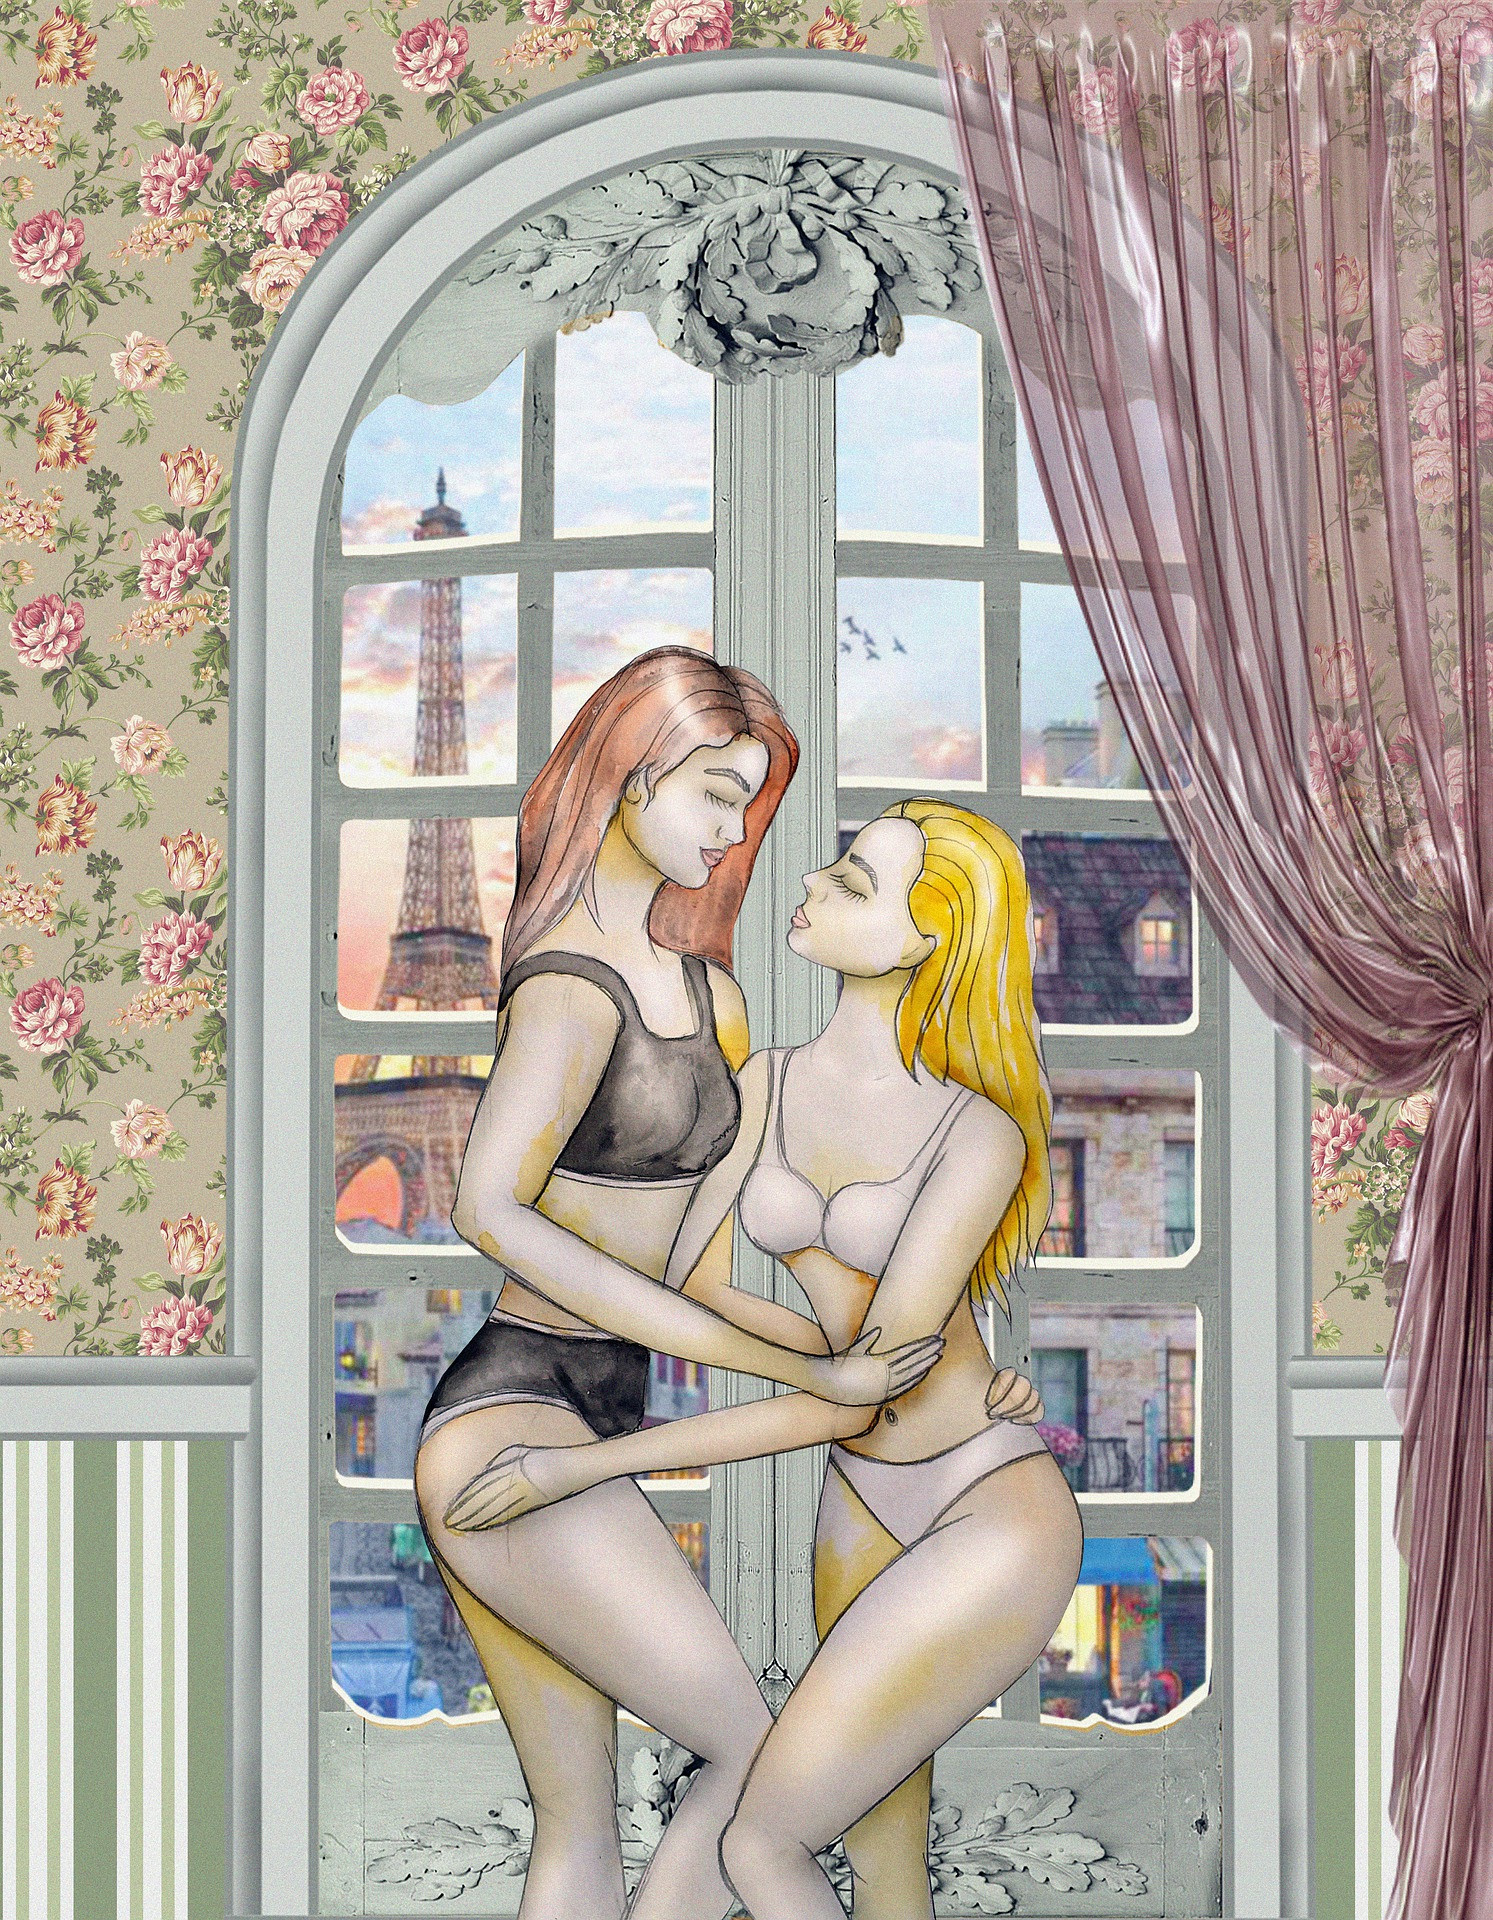
\includegraphics[width=1\textwidth]{images/brev76.png}
    \end{center}
}

%% CATEGORIES %%
\newcommand{\aBoire}{A boire}
\newcommand{\etudiant}{Etudiant}
\newcommand{\grenoble}{Grenoble}
\newcommand{\grivois}{Grivois}
\newcommand{\explicite}{Explicite}
\newcommand{\milimarin}{Milimarin}
\newcommand{\parodie}{Parodie}
\newcommand{\regional}{Regional}
\newcommand{\crado}{Crade}
\newcommand{\sentimental}{Sentimental}
\newcommand{\autre}{Autre}

\newCategory{\aBoire}
%\newCategory{A partition} Better to use a tag to only show songs with partition
\newCategory{\etudiant}
\newCategory{\grenoble}
\newCategory{\grivois}
\newCategory{\explicite}
\newCategory{\milimarin}
\newCategory{\parodie}
\newCategory{\regional}
\newCategory{\crado}
\newCategory{\sentimental}
\newCategory{\autre}

% Setting up commentary format as subsections

\breakpage

\insertChant{la-faluche}{paper}{\etudiant}
\insertChant{ave-le-petit-doigt}{paper}{\etudiant}
\insertChant{gaudeamus-igitur}{paper}{\etudiant}

\newSection{HYMNES DES FILIERES GRENOBLOISES}

\insertChantWithColor{chant-des-ingenieurs-grenoblois}{paper}{falRoyalBlue}{\etudiant, \grenoble}
\insertChantWithColor{la-pine-en-rose}{paper}{falPink}{\etudiant, \grenoble, \explicite}
\insertChantWithColor{chant-des-pharmaciens}{paper}{falGreen}{\etudiant, \grenoble, \explicite}
\insertChantWithColor{cesarise-la}{paper}{falFuchsia}{\etudiant, \grenoble, \crado}
\insertChantWithColor{hymne-des-sages-femmes}{paper}{falFuchsia}{\etudiant, \grenoble, \explicite}
\insertChantWithColor{l-hymne-juriste-grenoble}{paper}{falRed}{\etudiant, \grenoble}
\insertChantWithColor{l-hymne-interfilieres-grenoble}{paper}{falGrey}{\etudiant, \grenoble, \aBoire}
\insertChantWithColor{quand-les-sciences-s-en-vont-au-ppm}{paper}{falPurple}{\etudiant, \grenoble}

\newSection{PAILLARDIER}

\insertChant{51-je-t-aime}{paper}{\aBoire}
\insertChant{adam-et-eve}{onlineOnly}{\explicite}
\insertChant{adieu-fais-toi-putain}{paper}{\explicite}
\insertChant{adishatz}{paper}{\regional}
\insertChant{a-fond-liegeois}{onlineOnly}{\explicite}
\insertChant{ah-c-qu-on-est-bien}{paper}{\aBoire, \parodie}
\insertChant{ah-La-salope}{onlineOnly}{\explicite}
\insertChant{ah-le-petit-vin-blanc}{paper}{\aBoire}
\insertChant{ah-que-nos-peres}{paper}{\aBoire}
\insertChant{ah-si-tu-pouvais-fermer-ta-gueule}{onlineOnly}{\autre}
\insertChant{ah-viens}{paper}{\grivois}
\insertChant{ah-vous-dirais-je-maman}{onlineOnly}{\explicite}
\insertChant{a-la-claire-fontaine}{onlineOnly}{\explicite}
\insertChant{alcoolo}{paper}{\aBoire, \parodie}
\insertChant{les-aleas-de-l-amour}{paper}{\explicite}
\insertChant{alexandre}{paper}{\aBoire}
\insertChant{a-l-hopital-saint-louis}{paper}{\crado}
\insertChant{ali-pacha}{onlineOnly}{\explicite}
\insertChant{alka-seltzer}{onlineOnly}{\parodie, \explicite}
\insertChant{allons-a-messine}{onlineOnly}{\explicite}
\insertChant{alphonse-du-gros-caillou}{paper}{\grivois}
\insertChant{amis-buvons}{paper}{\aBoire}
\insertChant{l-ancien-etudiant}{paper}{\etudiant, \aBoire}
\insertChant{l-anus}{onlineOnly}{\explicite, \crado, \parodie}
\insertChant{l-apero-et-l-impetrant}{paper}{\etudiant, \aBoire, \parodie}
\insertChant{l-artilleur-de-metz}{paper}{\explicite, \milimarin}
\insertChant{a-trianon}{paper}{\grivois}
\insertChant{au-31-du-mois-d-aout}{paper}{\milimarin}
\insertChant{au-bal-de-l-hotel-dieu}{paper}{\explicite}
\insertChant{l-auberge-de-l-ecu}{paper}{\grivois}
\insertChant{au-clair-de-la-lune}{onlineOnly}{\explicite, \parodie}
\insertChant{aupres-de-ma-blonde}{paper}{\sentimental, \milimarin}
\insertChant{aussitot-que-la-lumiere}{paper}{\aBoire}
\insertChant{la-ballade-des-cocus}{paper}{\etudiant, \grivois}
\insertChant{le-bateau-des-vits}{onlineOnly}{\explicite}
\insertChant{bel-alcindor}{onlineOnly}{\explicite}
\insertChant{la-belle-et-le-cantonnier}{onlineOnly}{\parodie, \explicite}
\insertChant{belle-eugenie}{paper}{\regional, \grenoble, \sentimental}
\insertChant{benjamin}{paper}{\explicite}
\insertChant{les-betises}{onlineOnly}{\explicite, \crado, \parodie}
\insertChant{le-bicetre}{paper}{\explicite, \autre}
\insertChant{la-biere}{paper}{\aBoire}
\insertChant{la-biere-brel}{paper}{\aBoire}
\insertChant{billy-le-bordelais}{paper}{\aBoire, \grivois}
\insertChant{la-bite-noire}{onlineOnly}{\parodie, \explicite}
\insertChant{la-blanche-hermine}{paper}{\milimarin, \regional}
\insertChant{boire-un-petit-coup}{paper}{\aBoire, \grivois}
\insertChant{bois-de-l-arbois}{paper}{\aBoire, \regional}
\insertChant{la-boite-a-caca}{onlineOnly}{\explicite, \crado}
\insertChant{la-boiteuse}{paper}{\grivois}
\insertChant{le-bon-roi-dagobert}{onlineOnly}{\parodie, \explicite}
\insertChant{le-bordel-dans-le-bois}{onlineOnly}{\explicite}
\insertChant{la-bourguignonne}{paper}{\aBoire, \regional}
\insertChant{la-branleuse-de-taureau}{onlineOnly}{\explicite}
\insertChant{les-burnes-comptent-pas-pour-des-prunes}{onlineOnly}{\parodie, \explicite}
\insertChant{c-est-a-boire-qu-il-nous-faut}{paper}{\aBoire, \grivois}
\insertChant{les-canuts}{paper}{\regional}
\insertChant{la-capote-anglaise}{paper}{\parodie, \explicite}
\insertChant{caroline-la-putain}{onlineOnly}{\explicite}
\insertChant{catin-catin-aimable-catin}{paper}{\regional, \grenoble, \sentimental}
\insertChant{la-ceinture}{onlineOnly}{\grivois, \autre}
\insertChant{les-cents-louis-d-or}{onlineOnly}{\explicite}
\insertChant{ceux-qui-sont-nes}{paper}{\aBoire, \etudiant}
\insertChant{chanson-a-boire}{paper}{\aBoire}
\insertChant{chanson-a-virer}{paper}{\milimarin}
\insertChant{le-chant-des-corsaires}{paper}{\milimarin}
\insertChant{le-chant-des-etudiants-wallons}{paper}{\regional, \etudiant, \aBoire}
\insertChant{chanteur-d-apero}{onlineOnly}{\autre}
\insertChant{chantons-pour-passer-le-temps}{paper}{\sentimental, \milimarin}
\insertChant{charlotte}{onlineOnly}{\explicite}
\insertChant{la-chartreuse}{paper}{\grenoble, \aBoire, \parodie}
\insertChant{chartreuse-a-mourir}{paper}{\grenoble, \aBoire, \parodie}
\insertChant{chevaliers-de-la-table-ronde}{paper}{\aBoire, \grivois}
\insertChant{cochon-de-moine}{onlineOnly}{\explicite}
\insertChant{le-cocu-de-parame}{paper}{\grivois}
\insertChant{la-coloniale}{onlineOnly}{\milimarin, \explicite}
\insertChant{la-complainte-des-filles-de-grenoble}{onlineOnly}{\grenoble, \explicite}
\insertChant{la-complainte-de-mandrin}{paper}{\grenoble}
\insertChant{le-con-et-la-bouteille}{paper}{\aBoire, \explicite}
\insertChant{le-cordonnier-pamphile}{paper}{\explicite, \crado}
\insertChant{la-corinne}{onlineOnly}{\explicite}
\insertChant{le-corsaire-le-grand-coureur}{paper}{\milimarin}
\insertChant{le-cosaque}{onlineOnly}{\parodie, \explicite}
\insertChant{les-cosaques}{paper}{\regional}
\insertChant{la-coupo-santo}{paper}{\regional}
\insertChant{la-couture-avec-du-fil}{paper}{\etudiant, \parodie}
\insertChant{creme-nivea}{onlineOnly}{\explicite, \parodie}
\insertChant{c-t-envie-d-baiser}{onlineOnly}{\explicite, \parodie}
\insertChant{la-danse-des-queutards}{onlineOnly}{\explicite, \parodie}
\insertChant{lou-dauphinois}{paper}{\regional, \grenoble}
\insertChant{debout-les-fals}{paper}{\etudiant, \grenoble, \aBoire, \parodie}
\insertChant{de-profundis-morpionibus}{paper}{\crado, \grivois}
\insertChant{de-sur-la-mer}{paper}{\milimarin}
\insertChant{la-digue-du-cul}{onlineOnly}{\explicite}
\insertChant{la-dispute-du-cul-et-du-con}{paper}{\explicite}
\insertChant{le-duc-de-bordeaux}{paper}{\autre}
\insertChant{le-duc-de-bordeaux-2}{onlineOnly}{\explicite}
\insertChant{dudule}{onlineOnly}{\explicite}
\insertChant{en-revenant-de-charenton}{onlineOnly}{\explicite}
\insertChant{en-revenant-de-paris}{onlineOnly}{\explicite}
\insertChant{en-revenant-du-piemont}{paper}{\milimarin, \grivois}
\insertChant{etoile-des-neiges}{paper}{\regional, \sentimental}
\insertChant{fais-moi-une-piperade}{onlineOnly}{\grivois}
\insertChant{faluchardes-d-abord}{paper}{\etudiant, \parodie}
\insertChant{fanchon}{paper}{\aBoire, \grivois}
\insertChant{la-farandole-des-cochones}{onlineOnly}{\explicite}
\insertChant{la-femme-du-vidangeur}{onlineOnly}{\explicite, \crado}
\insertChant{les-filles-de-camaret}{onlineOnly}{\explicite, \crado}
\insertChant{les-filles-de-la-rochelle}{paper}{\grivois}
\insertChant{les-filles-des-forges}{paper}{\grivois, \regional}
\insertChant{le-forban}{paper}{\milimarin}
\insertChant{le-forban-alt}{onlineOnly}{\milimarin}
\insertChant{les-fraises-et-les-framboises}{onlineOnly}{\explicite}
\insertChant{frere-la-guillaumette}{onlineOnly}{\explicite}
\insertChant{fric-pharma}{paper}{\etudiant}
\insertChant{le-grand-vicaire}{onlineOnly}{\explicite}
\insertChant{le-grenadier-de-flandre}{paper}{\milimarin, \explicite}
\insertChant{la-grenobloise}{paper}{\grenoble}
\insertChant{guerre-guerre-vente-vent}{paper}{\milimarin}
\insertChant{le-hussard-de-la-garde}{paper}{\milimarin, \explicite, \crado}
\insertChant{hymne-des-faluchards}{paper}{\etudiant, \aBoire, \parodie}
\insertChant{il-etait-une-bergere}{paper}{\parodie, \grivois}
\insertChant{il-etait-un-vaisseau-de-guerre}{onlineOnly}{\parodie, \grivois, \milimarin}
\insertChant{il-faut-boire}{paper}{\aBoire}
\insertChant{l-internatonale-du-cul}{onlineOnly}{\parodie, \explicite}
\insertChant{j-ai-deux-amours}{paper}{\aBoire}
\insertChant{jaune}{paper}{\aBoire, \regional}
\insertChant{je-l-aide-a-vomir}{paper}{\parodie, \aBoire}
\insertChant{jeanneton}{onlineOnly}{\grivois}
\insertChant{jean-francois-de-nantes}{paper}{\milimarin, \grivois}
\insertChant{jean-gilles}{onlineOnly}{\explicite}
\insertChant{je-me-lave}{onlineOnly}{\parodie, \explicite}
\insertChant{la-jeune-fille-du-metro}{paper}{\grivois}
\insertChant{le-jeune-homme-de-besancon}{paper}{\explicite}
\insertChant{la-jument-de-michao}{paper}{\regional}
\insertChant{la-haut-sur-la-colline}{paper}{\grivois}
\insertChant{le-lundi-en-levrette}{onlineOnly}{\parodie, \explicite}
\insertChant{le-marechal}{paper}{\grivois}
\insertChant{maree-basse}{paper}{\aBoire}
\insertChant{margot}{onlineOnly}{\explicite}
\insertChant{la-mariee}{onlineOnly}{\grivois}
\insertChant{marie-madeleine}{onlineOnly}{\autre}
\insertChant{medecine-c-est-fini}{paper}{\etudiant, \parodie}
\insertChant{medecine-grenoble}{onlineOnly}{\etudiant, \grenoble}
\insertChant{mener-la-vache-au-taureau}{paper}{\autre}
\insertChant{la-mere-a-papa}{onlineOnly}{\grivois}
\insertChant{les-moines-de-saint-bernardin}{paper}{\explicite, \autre}
\insertChant{mon-ancetre-gurdil}{paper}{\autre, \aBoire}
\insertChant{le-musee-d-athenes}{paper}{\parodie, \explicite}
\insertChant{nissa-la-bella}{paper}{\regional}
\insertChant{nous-sommes-les-faluchards}{onlineOnly}{\etudiant, \explicite}
\insertChant{nous-sommes-unis-par-la-verole}{onlineOnly}{\explicite, \crado}
\insertChant{les-nuits-d-une-demoiselle}{paper}{\explicite, \grivois}
\insertChant{oh-mon-berger-fidele}{paper}{\explicite}
\insertChant{ouessant}{paper}{\regional, \milimarin}
\insertChant{ouvre-la-fenetre-qu-on-respire-un-peu}{paper}{\grivois}
\insertChant{la-paimpolaise-originale}{paper}{\regional, \sentimental, \milimarin}
\insertChant{la-paimpolaise}{onlineOnly}{\parodie, \regional}
\insertChant{passant-par-paris}{paper}{\sentimental}
\insertChant{la-patrouille}{paper}{\explicite}
\insertChant{la-peau-de-couille}{paper}{\explicite, \crado, \etudiant}
\insertChant{pelot-d-hennebont}{paper}{\milimarin}
\insertChant{le-petit-gregory}{onlineOnly}{\autre}
\insertChant{le-petit-ricard}{paper}{\aBoire}
\insertChant{les-petits-oiseaux}{paper}{\etudiant, \regional}
\insertChant{les-petits-glands}{onlineOnly}{\parodie, \explicite}
\insertChant{la-piemontaise}{paper}{\sentimental, \milimarin}
\insertChant{pierre-de-grenoble}{paper}{\sentimental, \grenoble, \regional, \milimarin}
\insertChant{les-pipes-dans-les-champs}{onlineOnly}{\parodie, \explicite}
\insertChant{plaisir-d-amour}{onlineOnly}{\explicite}
\insertChant{le-plaisir-des-dieux}{paper}{\explicite, \crado}
\insertChant{un-poil-de-cul-sur-ma-savonette}{onlineOnly}{\crado}
\insertChant{la-pompe-a-merde}{paper}{\crado}
\insertChant{le-pou-et-l-araignee}{paper}{\grivois}
\insertChant{premature}{onlineOnly}{\parodie}
\insertChant{les-premices-de-l-amour-version-feminine}{onlineOnly}{\parodie, \explicite}
\insertChant{les-premices-de-l-amour-version-masculine}{onlineOnly}{\parodie, \explicite}
\insertChant{prendre-un-gros-gland}{onlineOnly}{\parodie, \explicite}
\insertChant{les-prisons-de-nantes}{paper}{\regional}
\insertChant{la-p-tite-huguette}{paper}{\explicite}
\insertChant{la-puce}{paper}{\grivois}
\insertChant{quand-je-bois-du-vin-clairet}{paper}{\aBoire}
\insertChant{les-quatre-vingt-chasseurs}{onlineOnly}{\grivois}
\insertChant{quinze-marins}{paper}{\milimarin}
\insertChant{qu-on-apporte}{paper}{\grivois}
\insertChant{rabats-ta-queue}{onlineOnly}{\crado, \explicite}
\insertChant{les-retrouvailles}{paper}{\aBoire, \sentimental}
\insertChant{reveillez-vous-picards}{paper}{\milimarin, \regional}
\insertChant{les-grenoblois}{onlineOnly}{\grenoble, \etudiant, \explicite}
\insertChant{du-rhum-des-femmes}{paper}{\aBoire, \grivois}
\insertChant{la-rue-cuvier}{paper}{\explicite}
\insertChant{sa-grande-pine}{onlineOnly}{\explicite}
\insertChant{santiano}{paper}{\milimarin}
\insertChant{la-semaine-etudiante}{onlineOnly}{\explicite}
\insertChant{le-semeur}{paper}{\etudiant, \regional}
\insertChant{le-soldat-belge}{paper}{\milimarin, \regional}
\insertChant{sommes-nous-des-grenouilles}{paper}{\aBoire, \autre}
\insertChant{sont-les-filles-de-la-rochelle}{paper}{\milimarin, \explicite}
\insertChant{sur-la-route-de-san-francisco}{paper}{\milimarin}
\insertChant{stances-a-sophie}{onlineOnly}{\explicite, \crado}
\insertChant{la-strasbourgeoise}{paper}{\milimarin, \regional}
\insertChant{tape-ta-pine}{onlineOnly}{\explicite}
\insertChant{le-temps-des-cerises}{paper}{\sentimental}
\insertChant{la-tirade-de-noeuds}{onlineOnly}{\parodie, \explicite}
\insertChant{torche-la-gueule-a-ton-voisin}{paper}{\aBoire}
\insertChant{la-tour-de-londres}{paper}{\explicite, \crado}
\insertChant{tous-les-chemins-menent-au-rhum}{paper}{\aBoire}
\insertChant{tous-les-pochtrons}{onlineOnly}{\aBoire, \parodie, \grenoble}
\insertChant{tout-sur-le-clito}{onlineOnly}{\parodie, \explicite}
\insertChant{le-tralala-de-la-mere-michel}{onlineOnly}{\explicite}
\insertChant{trent-six-matelots}{paper}{\milimarin, \sentimental}
\insertChant{les-trois-orfevres}{paper}{\explicite, \crado}
\insertChant{le-troubadour}{onlineOnly}{\explicite}
\insertChant{ursule}{onlineOnly}{\grivois, \crado, \parodie}
\insertChant{la-vache}{onlineOnly}{\autre}
\insertChant{le-vieux-cure-de-paris}{onlineOnly}{\grivois, \parodie}
\insertChant{le-vin-gaulois}{paper}{\milimarin}
\insertChant{viv-les-etudiants}{onlineOnly}{\etudiant, \explicite, \crado}
\insertChant{vive-les-etudiants}{onlineOnly}{\etudiant, \explicite}
\insertChant{vive-les-gros-nichons}{onlineOnly}{\explicite}
\insertChant{y-a-quatre-marins}{paper}{\milimarin}

\newSection{NOUVEAUTES}
\insertChant{propals/le-vrai-plaisir-des-dieux}{paper}{\explicite, \crado}
\insertChant{propals/la-maman-des-boissons}{paper}{\aBoire, \grenoble}


% \newpage
% \addcontentsline{toc}{section}{Code Grenoblois} \label{code-grenoblois}
% \includepdf[pages=1-26]{code_mini.pdf}

\sectionfont{\color{black}} 

\breakpage
% \let\section\oldsection
% \pdfbookmark{Contents}{Contents}
% \section*{Sommaire par catégorie} \label{sommaire}
% \addcontentsline{toc}{section}{Sommaire par catégorie} 
\section*{Sommaire par catégorie} \label{sommaire}
\noindent
\tagged{categories}{
    \phantomsection
    \printCategory{A boire}{Chants à boire}\label{sec:A boire}\phantomsection
    \vspace*{0.2cm}\blackline
    \printCategory{Etudiant}{Estudiantines}\label{sec:Etudiant}\phantomsection
    \vspace*{0.2cm}\tagged{onlineOnly}{\blackline}
    \printCategory{Grenoble}{De Grenoble}\label{sec:Grenoble}\phantomsection
    \vspace*{0.2cm}\untagged{onlineOnly}{\blackline}\tagged{onlineOnly}{\vspace{2cm}}
    \printCategory{Grivois}{Chansons grivoises}\label{sec:Grivois}\phantomsection
    \vspace*{0.2cm}\untagged{onlineOnly}{\blackline}
    \printCategory{Explicite}{Chansons explicites}\label{sec:Explicite}\phantomsection
    \vspace*{0.2cm}\blackline
    \printCategory{Milimarin}{Militaires et marins}\label{sec:Milimarin}\phantomsection
    \vspace*{0.2cm}\blackline
    \printCategory{Parodie}{Parodies}\label{sec:Parodie}\phantomsection
    \vspace*{0.2cm}\blackline
    \printCategory{Regional}{Chants régionaux}\label{sec:Regional}\phantomsection
    \vspace*{0.2cm}\blackline
    \printCategory{Crade}{Chants crades}\label{sec:Crade}\phantomsection
    \vspace*{0.2cm}\tagged{onlineOnly}{\blackline}
    \printCategory{Sentimental}{Sentimentales}\label{sec:Sentimental}\phantomsection
    \vspace*{0.2cm}\tagged{paper}{\blackline}
    \printCategory{Autre}{Autre}\label{sec:Autre}\phantomsection
}

\breakpage
% \let\section\oldsection
% \pdfbookmark{Contents}{Contents}
% \section*{Remerciements} \label{Remerciements}
% \addcontentsline{toc}{section}{Remerciements} 
\section*{Remerciements} \label{Remerciements}
\noindent

\textbf{Pour le travail repris de la dernière édition du bréviaire}

\textit{Dessins:}
\begin{addmargin}[1em]{2em}% 1em left, 2em right
6Lance, Crocaïne et Playmobite <3{\color{falGrey!60!black}, Sciences Grenoble}
\\Craziiiii{\color{falGrey!60!black}, Droit Grenoble}
\\JCVD et Mogwai{\color{falGrey!60!black}, Ingénieur.e.s Grenoble}
\\Minionidas{\color{falGrey!60!black}, Jaune Grenoble}
\\MimiGeignarde{\color{falGrey!60!black}, IAE Toulouse}
\\Mr Colle{\color{falGrey!60!black}, Médecine Grenoble}
\\Sonic{\color{falGrey!60!black}, Jaune Valence}\\
\end{addmargin}

\textit{Mise en page et rédaction:}
\begin{addmargin}[1em]{2em}% 1em left, 2em right
6Lance et Crocaïne{\color{falGrey!60!black}, Sciences Grenoble}\\
\end{addmargin}

\bigskip
\textbf{Pour le travail effectué sur cette édition}

\textit{Notation des chants à ajouter/enlever:}
\begin{addmargin}[1em]{2em}% 1em left, 2em right
<3Beer, Lucie, Spatt0une, Calondorf, Panoramix, Morgane, Tiphaine et Gringotts{\color{falGrey!60!black}, Ingénieur.e.s Grenoble}
\\Sirius3{\color{falGrey!60!black}, Jaune Grenoble}
\\Hector{\color{falGrey!60!black}, Sciences Grenoble}
\\Louis{\color{falGrey!60!black}, impétrant Sciences Cler-noble}
\\RiGHor MortiX{\color{falGrey!60!black}, Rose Grenoble}\\
\end{addmargin}

\textit{Partitions et investissement général:}
\begin{addmargin}[1em]{2em}% 1em left, 2em right
Lucie{\color{falGrey!60!black}, Ingénieure Grenoble}\\
\end{addmargin}

\textit{Recherches sur les chants et investissement général:}
\begin{addmargin}[1em]{2em}% 1em left, 2em right
<3Beer{\color{falGrey!60!black}, Ingénieur Grenoble}\\
\end{addmargin}

\textit{Mise en page}
\begin{addmargin}[1em]{2em}% 1em left, 2em right
Spatt0une{\color{falGrey!60!black}, Ingénieur Grenoble}\\
\end{addmargin}

\textbf{Un grand merci à Xavier Hubaut, Professeur émérite du Département de Mathématique (Université Libre de Bruxelles), pour le travail d'archives et de recherches effectué et dont nous tenons une certaine part des commentaires de ce bréviaire.}

\end{document}